\documentclass[11pt]{beamer}
\usetheme{CambridgeUS}
\usepackage[utf8]{inputenc}
\usepackage{amsmath}
\usepackage{amsthm}
\usepackage{amsfonts}
\usepackage{amssymb}
\usepackage{graphicx}
\usepackage{pgfpages}
\usepackage{framed}
\usepackage{multicol}
\usepackage{etoolbox}
\usepackage{lipsum}

\theoremstyle{plain} 
\newtheorem{thm}{Theorem}[section] 
\newtheorem{cor}[thm]{Corollary} 
\newtheorem{lem}[thm]{Lemma} 
\newtheorem{prop}[thm]{Proposition} 
\theoremstyle{definition} 
%\newtheorem{defn}{Definizione}[chapter] 
\theoremstyle{remark} 
\newtheorem{oss}{Osservazione} 

\AtBeginSection[]{
  \begin{frame}
  \vfill
  \centering
  \begin{beamercolorbox}[sep=8pt,center,shadow=true,rounded=true]{title}
    \usebeamerfont{title}\insertsectionhead\par%
  \end{beamercolorbox}
  \vfill
  \end{frame}
}

\author{Giovanni Della Lunga}
\title{Modelling Dependence with Copulas}
\subtitle{An Introduction} % (optional)
\setbeamercovered{transparent} 
%\setbeamertemplate{navigation symbols}{} 
%\logo{} 
\institute{WORKSHOP IN QUANTITATIVE FINANCE} 
\date{Bologna - May 3-4, 2018} %\subject{} 
\begin{document}

\begin{frame}
\titlepage
\end{frame}

\makeatletter
\patchcmd{\beamer@sectionintoc}
  {\vfill}
  {\vskip2.5\itemsep}
  {}
  {}
\makeatother 

\begin{frame}
\frametitle{Outline}
  \begin{multicols}{2}
  \tableofcontents
  \end{multicols}
\end{frame}

%===================================================================================================
\section{Introduction}

%___________________________________________________________________________________________________
%
\begin{frame}{Introduction}
   %\footnotesize{
   \begin{itemize}
      	\item  Many real-life situations can be modelled by a large number of random variables which play a significant role, and such 
      	variates are generally not independent. 
		\item Therefore, it is often of fundamental importance to be able to link the marginal distributions of different variables in order 
		to give a flexible and accurate descrip- tion of the joint law of the variables of interest. 	
		\item Copulas were introduced in 1959 in the context of probabilistic metric spaces and later exploited as a tool for 
		understanding relationships among multivariate outcomes. 
		\item A copula is a function that links univariate marginals to their joint multivariate distribution in such a way that it captures 
		the entire dependence structure in the multivariate distribution. 
   \end{itemize}
 %  }
\end{frame}
%___________________________________________________________________________________________________
%
\begin{frame}{Introduction}
   %\footnotesize{
   \begin{itemize}
		\item The main advantage provided by a copula-approach in dependence modelling is that the selection of an appropriate model 
		for the dependence between variables X and Y , represented by the copula, can proceed independently from the choice of the 
		marginal distributions. 
		\item The seminal result in the history of copulas is due to Sklar that introduced in 1959 the notion, and the name, of copula, 
		and proved the theo- rem that now bears his name (Sklar, 1959). 
		\item The latter states that any multivariate distribution can be expressed as its copula function evaluated at its marginal 
		distribution functions. 
		\item Moreover, any copula function when evaluated at any marginal distributions is a multivariate distribution.
   \end{itemize}
 %  }
\end{frame}
%___________________________________________________________________________________________________
%
\begin{frame}{Introduction}
		\begin{itemize}
		\item This presentation is so organized: 
		in section 2 we recall some basic concepts from multivariate distributions theory, after Section 3 in which we define 
		the concept of copula in full generality, we turn in Section 4 to an overview of the most important notions of 
		dependence used in IRM. Section 5 introduces the most important families of copulas, their properties both 
		methodological as well as with respect to simulation. Finally in Section 6 we discuss the concept of tail dependence.
		\item
		I would like to stress that this presentation only gives a first introduction, topics not included are statistical 
		estimation of copulas and the modelling of dependence, through copulas, in a dynamic environment.
		\end{itemize}
\end{frame}
%___________________________________________________________________________________________________
%
\begin{frame}{The Problem (Embrechts, 2009)}
   %\footnotesize{
	\noindent\begin{minipage}{0.5\textwidth}% adapt widths of minipages to your needs
	
\includegraphics[width=\linewidth]{fig/omino_interrogativo.png}
	\end{minipage}%
	\hfill%
	\begin{minipage}{0.5\textwidth}
	   \begin{itemize}
	      \item A problem well known by all those who deal with Risk Management is the following: "Here we are given a multi-
	      dimensional (i.e. 
	      several risk factors) problem for which we have marginal information together with an idea of dependence". 
		  \item Now the question is: \textbf{When is this problem well-posed?}
	   \end{itemize}
	 %  }
	\end{minipage}
\end{frame}
%___________________________________________________________________________________________________
%
\begin{frame}{The Problem (Embrechts, 2009)}
   %\footnotesize{
   \begin{itemize}
      \item  One concrete question could be this: given two marginal, one-period risk factors $X_1$ ed $X_2$ with lognormal distribution 
      functions (dfs) 
       $F_1 = LN(\mu=0, \sigma=1)$ and  $F_1 = LN(\mu=0, \sigma=4)$. How can we simulate from such a model if $X_1$ and $X_2$ 
       have linear correlation $\rho = 0.5$ say?
	  \item First of all, the correlation information say something (but what?) about the bivariate df of the random vectors $(X_1, X_2)^T$, 
	  i.e. about
	    $F(x_1, x_2) = Prob[x_1 \le X_1, x_2 \le X_2]$;
	  \item Note however that, in the above, that information is \textbf{not} given; we \textbf{only} know $F_1$, $F_2$ e $\rho$; 
	  \item What else would one need?
   \end{itemize}
 %  }
\end{frame}
%___________________________________________________________________________________________________
%
\begin{frame}{The easy Copula argument}
   %\footnotesize{
   \begin{itemize}
	    \item First note that for random variables (rvs) $X_i$ with continuous dfs $F_i$, le variabili $U_i= F_i(X_i) $ are uniformly distributed 
	    rvs on $[0, 1]$;
		\item Hence for some joint df $F$ with marginal dfs $F_1$ e $F_2$ we have:
		\begin{equation}
			\begin{split}
			F(X_1, X_2) &= P(X_1 \le x_1, X_2 \le x_2) \\
			&= P(F_1(X_1) \le F_1(x_1), F_1(X_2) \le F_1(x_2)) \\
			&= P(U_1 \le F_1(x_1), U_2 \le F_2(x_2)) \\
			& := C(F_1(x_1), F_2(x_2)) 
			\end{split}
		\end{equation}	  
		\item The function $C$ above is exactly \textit{a} (careful here!) \textbf{copula}, a df on $I^2 = [0, 1] \times [0, 1]$ with standard 
		uniform marginals, $C$ is the df of the random vector $(U_1, U_2)^T$.  
   \end{itemize}
 %  }
\end{frame}
%___________________________________________________________________________________________________
%
\begin{frame}{The easy Copula argument}
   %\footnotesize{
   \begin{itemize}
      \item  If we return to our lognormal example, we see no immediate reason how the number $\rho$ should determine the function $C$, 
      it is not even clear whether the problem has none, one or infinitely many solutions;
      \item In this case, it turns out that the problem posed has \textbf{no} solution.  				  						  
      \item The time has come to move on to some definition ... 
   \end{itemize}
 %  }
\end{frame}
%===================================================================================================
\section{Joint Distributions}
%___________________________________________________________________________________________________
%
\begin{frame}{Distribution Function}
   %\footnotesize{
   \begin{itemize}
      \item  Lets take a random real value array $X=(X_1, \dots, X_d)$ we can define a multivariate distribution function $F$:
		$$F(\mathbf{x}) = Prob[X_1 \le x_1, \dots, X_d \le x_d]$$
	   \item In general a distribution function $F$ defined from $\mathbb{R}$ in $I$, must meet the following conditions:
		\begin{itemize}
			\item $F(x) \ge 0 \quad \forall x$
			\item $\lim\limits_{x_i \rightarrow +\infty} F(x_1,\dots,x_d) =1 \quad \forall x_i$
			\item $\lim\limits_{x_i \rightarrow -\infty} F(x_1,\dots,x_d) = 0 \quad \forall x_i$
		\end{itemize}	  
   \end{itemize}
 %  }
\end{frame}
%___________________________________________________________________________________________________
%
\begin{frame}{Distribution Function}

\noindent\begin{minipage}{0.5\textwidth}% adapt widths of minipages to your needs
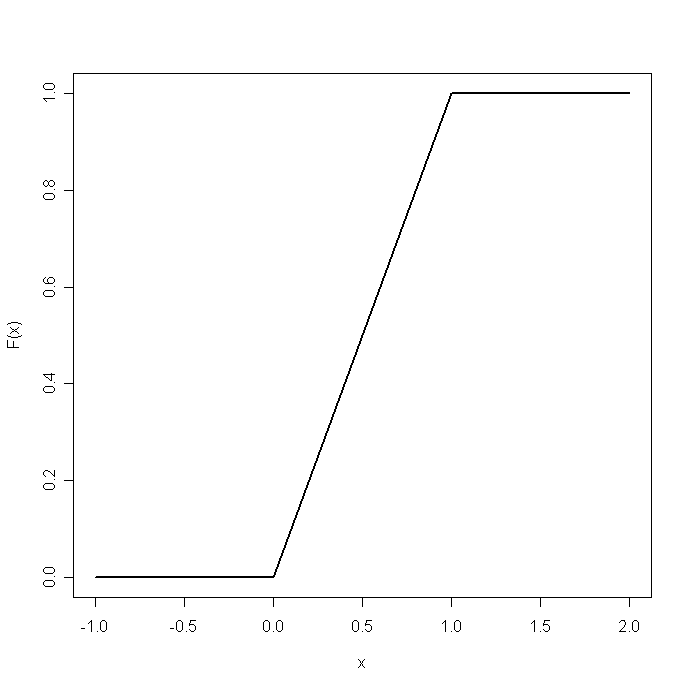
\includegraphics[width=\linewidth]{fig/cumulata_uniforme.png}
\end{minipage}%
\hfill%
\begin{minipage}{0.5\textwidth}
	\begin{itemize}
		\item Let $\mathbf{X}$ be a uniform random variable $[0, 1]$, the distribution function is: 
		\begin{equation*}
		    F(x) = \begin{cases}
		               0               & x < 0\\
		               x               & 0 \le x < 1\\
		               1               & x = 1
		           \end{cases}
		\end{equation*}
	\end{itemize}
\end{minipage}
\end{frame}
%___________________________________________________________________________________________________
%
\begin{frame}{Joint Cumulative Distribution Function}
	Remember that the \textbf{joint cumulative function} of two random variables $X$ and $Y$ 	is defined as
	\begin{equation}
			F_{XY}(x,y)= \mathbb{P}(X \leq x, Y \leq y)
	\end{equation}
	The joint CDF satisfies the following properties:
    \footnotesize{
    \begin{enumerate}
      	\item   				  						  
		$F_X(x)=F_{XY}(x, \infty)$, for any $x$ (marginal CDF of $X$); 
	  	\item 
	  	$F_Y(y)=F_{XY}(\infty,y)$, for any $y$ (marginal CDF of $Y$);
		\item 
		$F_{XY}(\infty, \infty)=1$;
		\item
		$F_{XY}(-\infty, y)=F_{XY}(x,-\infty)=0$;
		\item
		$\mathbb{P}(x_1 < X \leq x_2, \hspace{5pt} y_1  <Y \leq y_2)=$
        $F_{XY}(x_2,y_2)-F_{XY}(x_1,y_2)-F_{XY}(x_2,y_1)+F_{XY}(x_1,y_1)$;
        \item
        if $X$ and $Y$ are independent, then $F_{XY}(x,y)=F_X(x)F_Y(y)$.
   \end{enumerate}}
\end{frame}
%___________________________________________________________________________________________________
%
\begin{frame}{Joint Cumulative Distribution Function}
		In particular from property 5, putting $x_2 \rightarrow +\infty$ and $y_2 
		\rightarrow +\infty$ we have
			\begin{equation}
			\begin{split}
			\mathbb{P}(x_1 < X \leq +\infty, \hspace{5pt} y_1  <Y \leq +\infty) & =
			     F_{XY}(+\infty,+\infty)-F_{XY}(x_1,+\infty) \\
			     & -F_{XY}(+\infty,y_1)+F_{XY}(x_1,y_1)      \\
			& = 1 - F_X(x) - F_Y(y) + F_{XY}(x_1,y_1)     
			\end{split}
			\end{equation}
        
		If we denote with $\bar F_{XY}(x, y ) = \mathbb{P}[X > x, Y > y]$, we finally obtain
		
		\begin{equation}
		\bar F_{XY}(x, y ) = 1 - F_X(x) - F_Y(y) + F_{XY}(x, y)
		\end{equation}
\end{frame}

%===================================================================================================
\section{Copulas}
%___________________________________________________________________________________________________
%
\begin{frame}{Copulas}
   %\footnotesize{
   \begin{itemize}
   		\item The concept of \textbf{copula} arises from the idea of breaking down a multivariate distribution $F$ into components allow one 
   		to easily model and estimate the distribution of random vectors by estimating marginals and dependency structure separately;
	  	\item The importance of the copula functions derives entirely from a noteworthy result known in the literature as \textbf{Sklar's 
	  	theorem} that states that any multivariate joint distribution can be written in terms of univariate marginal distribution functions and a 
	  	copula which describes the dependence structure between the variables;
	 	\item Before discussing the theorem we are gong to describe some of the fundamental properties of copula functions limiting (for 
	 	simplicity) to the bivariate case and recalling our \textit{definition} of copula function as a bi-variate distribution of two marginally 
	 	uniform variables ...
   \end{itemize}
 %  }
\end{frame}
%___________________________________________________________________________________________________
%
\begin{frame}{Copulas}
  \footnotesize{
   \begin{itemize}
      \item   				  						  
			According to our previous definition
			\begin{equation}\label{copula_1}
				C(x,y) = P(U_1 \le x, U_2 \le y)
			\end{equation}		 
	  \item From the above equation we can write:
			  \begin{equation}\label{copula_2}
					  \begin{split}
					  &C(x,0) = P(U_1 \le x, U_2 \le 0) = 0 \\
					  &C(0,y) = P(U_1 \le 0, U_2 \le y) = 0 \\
					  &C(x,1) = P(U_1 \le x, U_2 \le 1) = P(U_1 \le x) = x \\
				      &C(1,y) = P(U_1 \le 1, U_2 \le y) = P(U_2 \le y) = y	   
					  \end{split}	   
			  \end{equation}
	\item in particular from the last two relations of \eqref{copula_2} we obtain
			\begin{equation}\label{copula_3}
					C(x,y) \le C(x,1) = x \quad C(x,y) \le C(1,y) = y \Rightarrow C(x,y) \le \min(x,y)
			\end{equation}
   \end{itemize}
 }
\end{frame}
%___________________________________________________________________________________________________
%
\begin{frame}{Copulas}
\noindent
\begin{minipage}{0.5\textwidth}% adapt widths of minipages to your needs
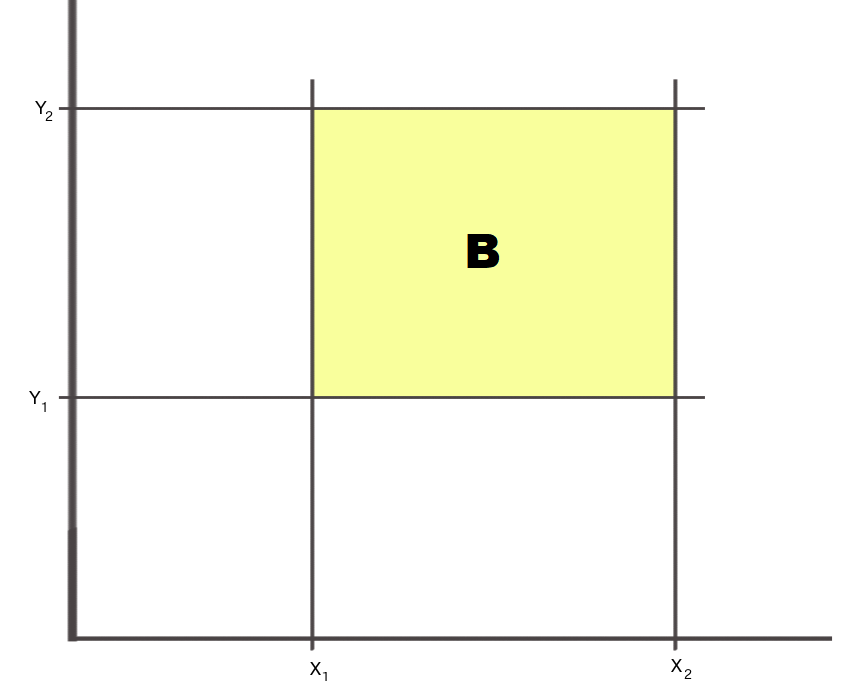
\includegraphics[width=\linewidth]{fig/copula_definizione_quadrato.png}
\end{minipage}%
\hfill%
\begin{minipage}{0.5\textwidth}
		\begin{itemize}
				\item The volume of the square in the picture is clearly equal to
						\begin{equation}
								\begin{split}
								& V([x_1, x_2] \times [y_1, y_2]) = \\
								& (x_2-x_1)\cdot (y_2-y_1) = \\
								& x_2y_2 - x_2y_1 -x_1y_2 + x_1y_1
								\end{split}
						\end{equation}
				\item Generaly speaking, for each function $H$ we can define a generalized-volume or \textit{H-Volume} by:
						\begin{equation}
								\begin{split}
								V_H(B) &= H(x_2,y_2) -H( x_2,y_1) \\
								&- H(x_1,y_2) + H( x_1,y_1)
								\end{split}
						\end{equation}
		\end{itemize}
\end{minipage}
\end{frame}
%___________________________________________________________________________________________________
%
\begin{frame}{Copulas}
   %\footnotesize{
   \begin{itemize}
      \item   				  						  
		For the C-Volume to be considered as a probability, it must be always positive 
		definite 
		\begin{equation}
			  C(x_2, y_2) - C(x_2, y_1) - C(x_1, y_2) + C(x_1, y_1) \ge 0
		\end{equation}	  	
	  \item 
	  	This must be true however the four values $x_i$, $y_i$ are chosen, in particular if 
	  	we choose $(x_2, y_2) = (x,y)$ e $(x_1,y_1)=(1,1)$ we have
		\begin{equation}
				  C(x, y) - C(x,1) - C(1,y) + C(1,1) \ge 0
		\end{equation}
	\item 
		Remember that $C(x,1)=x$ e $C(1,y) = y$, so we have $C(x,y) \ge x+y-1 $ and $C(x,y) 
		\ge 0$ then:
		\begin{equation}\label{copula_4}
					C(x,y) \ge \max(x+y-1,0) 
		\end{equation}
\end{itemize}
 %  }
\end{frame}
%___________________________________________________________________________________________________
%
\begin{frame}{Fréchet Limits}
   %\footnotesize{
   \begin{itemize}
   		\item  Putting together \eqref{copula_4} and \eqref{copula_3} we have 
				\begin{equation}
				 \max(x+y-1,0) \le C(x,y) \le \min(x,y)
				\end{equation}
	  	\item This is a special case of one of the most important results of multivariate statistics the\textbf{Fréchet-
	  	Hoeffding Theorem}.

		\begin{thm}[Fréchet-Hoeffding Bounds]
          	Suppose $F_1,\dots, F_d$ are marginal dfs and  $F$ any joint df with those given marginals, then 
          	$\forall \mathbf{x} \in \mathbb{R}^d$,
					\begin{equation}
					\Bigl( 
					\sum\limits_{k=1}^d  F_k(x_k) + 1 -d
					\Bigr)^+
					\le F(\mathbf{x}) \le 
					\min(F_1(x_1),\dots,F_d(x_d))
					\end{equation}
		\end{thm}
   \end{itemize}
 %  }
\end{frame}
%___________________________________________________________________________________________________
%
\begin{frame}{Fréchet Limits}
    \begin{figure}[ht]
        \begin{minipage}[b]{0.45\linewidth}
            \centering
            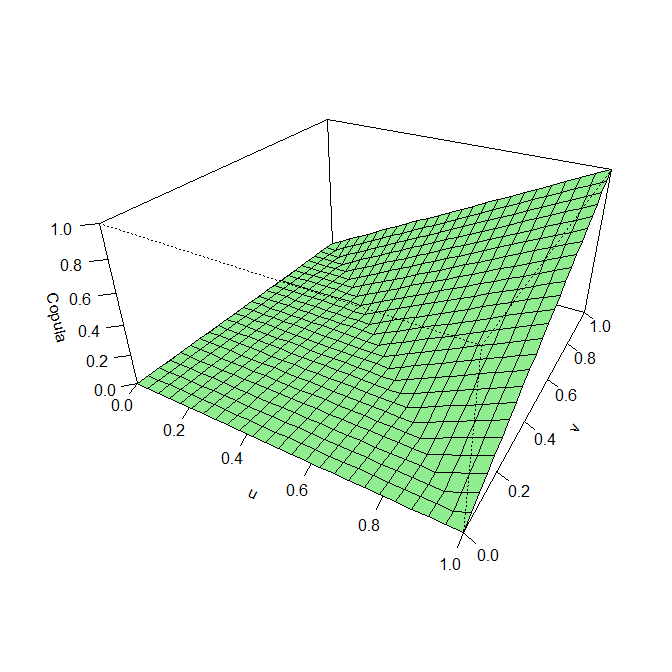
\includegraphics[width=\textwidth]{fig/copula_minima.png}
            \caption{a) Minimum Copula}
            \label{fig:a}
        \end{minipage}
        \hspace{0.5cm}
        \begin{minipage}[b]{0.45\linewidth}
            \centering
            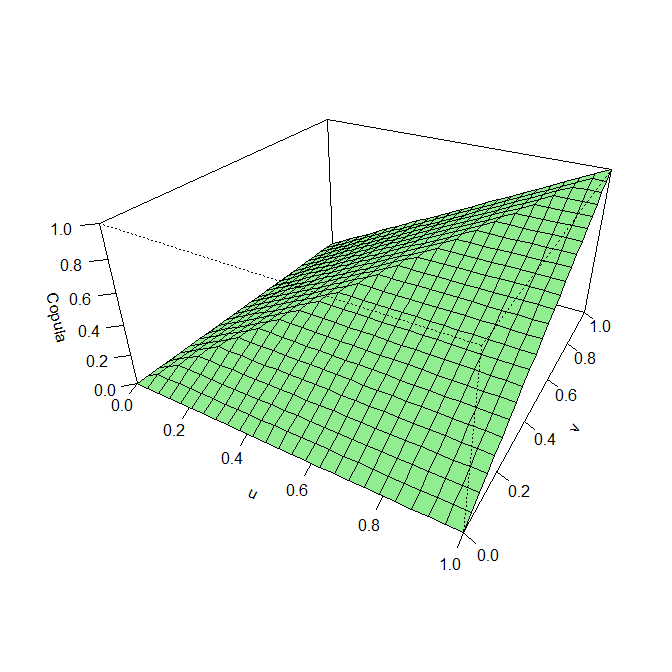
\includegraphics[width=\textwidth]{fig/copula_massima.png}
            \caption{b) Maximum Copula}
            \label{fig:b}
        \end{minipage}
    \end{figure}
\end{frame}
%___________________________________________________________________________________________________
%
\begin{frame}{Sklar's Theorem}
   %\footnotesize{
   \begin{itemize}
      \item  The key to link copula functions and distribution functions is represented by the \textbf{Sklar Theorem}:
	  \begin{thm}[A. Sklar, 1959]
			Suppose $X_1, \dots, X_d$ are rvs with continuous dfs $F_1, \dots, F_d$ and joint df $F$, then there exists a unique copula $C$ 
			(a df on $[0, 1]^d$ with uniform marginals) such that for all $\mathbf{x} \in \mathbb{R}^d$: 
					\begin{equation}\label{sklar_1}
							F(x_1,\dots,x_d) = C(F_1(x_1),\dots,F_d(x_d))
					\end{equation}
			Conversely given any dfs $F_1, \dots, F_d$ and copula $C$, $F$ defined through \eqref{sklar_1} is a d-variate df with marginal dfs  
			$F_1,\dots,F_d$.
	\end{thm} 
   \end{itemize}
 %  }
\end{frame}
%___________________________________________________________________________________________________
%
\begin{frame}{Sklar's Theorem}
   %\footnotesize{
   \begin{itemize}
      \item 
      	The theorem guarantees that for continuous random variables, the univariate margins 
      	and the multivariate dependence structure can be univocally separated and that the 
      	copula fully describes the dependence structure;  				  							  \item 
      	The theorem can be reversed, so that the copula can be described in terms of a joint 
      	distribution function and quantile functions of the marginal ones.
		\begin{cor}
			Let be $F, F_1, \dots, F_d$ and $C$ the same as in Sklar Theorem and $F_1^{-1}, 
			\dots, F_d^{-1}$ the quantile functions of $F_1, \dots, F_d$ then we can write:
			\begin{equation}\label{sklar_2}
							C(\mathbf{u}) = F(F_1^{-1}(u_1), \dots, F_d^{-1}(u_d)) 
			\end{equation}  
		\end{cor} 
   \end{itemize}
 %  }
\end{frame}
%___________________________________________________________________________________________________
%
\begin{frame}{Independence}
	\noindent
	\begin{minipage}{0.5\textwidth}% adapt widths of minipages to your needs
	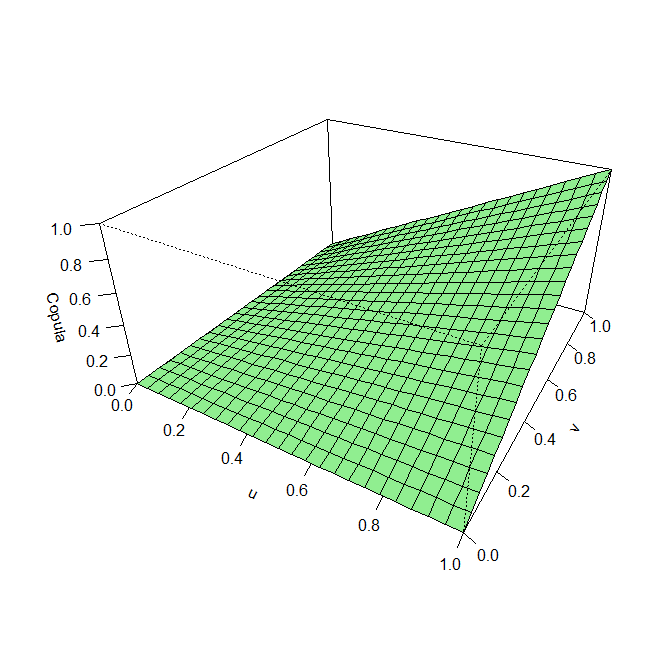
\includegraphics[width=\linewidth]{fig/copula_prodotto.png}
	\end{minipage}%
	\hfill%
	\begin{minipage}{0.5\textwidth}
	\begin{itemize}
		\item Also the concept of independence between random variables can be represented in terms of copulas;
		\item In terms of copulas, if the random variables are independent, the functional that describes the link between the marginal 
		distribution functions and the joint one is the product copula, conversely if some variables are associated with the product copula then
		they are independent
	\end{itemize}
	\end{minipage}
\end{frame}


\subsection{Survival Copula}
%___________________________________________________________________________________________________
%
\begin{frame}{Survival Copula}
   %\footnotesize{
   \begin{itemize}
      \item   				  						  
		The survival copula associated with the copula $C$ is
			\begin{equation}
			\bar C (u, v) = u + v - 1 + C(1-u, 1-v)
			\end{equation}
	  \item 
	  	It is easy to verify that $\bar C$ ha the copula properties. Once computed in $(1-u 
	  	,1-v)$ is equivalent to the complementary distribution function of a bivariate 
	  	uniform distribution, since
		\begin{equation}
			\begin{split}
			\bar C (1-u, 1- v) & = 1 - u + 1 - v - 1 + C(u, v) \\
			& = 1 - \mathbb{P} (U_1 \le u) + 1 - \mathbb{P} (U_2 \le v) - 1 \\
			& + \mathbb{P} (U_1 \le u, U_2 \le v) \\
			& = 1 - \mathbb{P} (U_1 \le u) - \mathbb{P} (U_2 \le v) + \mathbb{P} (U_1 \le u, 
			U_2 
			\le v) \\
			& = \mathbb{P} (U_1 > u, U_2 > v)
			\end{split}
	  	\end{equation}	  	
   \end{itemize}
 %  }
\end{frame}

\subsection{Density}
%___________________________________________________________________________________________________
%
\begin{frame}{Density}
   %\footnotesize{
   \begin{itemize}
      \item   				  						  
			If $C$ is absolutely continuous then it can be written in the form 
			
			\begin{equation}
			C(\mathbf{u}) = \int\limits_{[0, \mathbf{u}]^d} c(\mathbf{s}) \> d \mathbf{s}
			\end{equation}
			
			where $c$ is a suitable function called \textit{density} of $C$. 
	  \item 
	  		In particular, for almost all $\mathbf{u} \in \mathbb{I}^d$ one has
	  		\begin{equation}
				c(\mathbf{u}) = \frac{\partial^d C(\mathbf{u})}{\partial u_1 \dots \partial 
				u_d}
			\end{equation}
	  \item 
			As stressed by many authors, this equation is far from obvious. In fact, there 
			are some facts that are implicitly used: first, the mixed partial derivatives of 
			order $d$ of $C$ exist and are equal almost everywhere on $\mathbb{I}^d$; second 
			each mixed partial derivative is actually almost everywhere equal to the density 
			$c$. 
   \end{itemize}
 %  }
\end{frame}
%___________________________________________________________________________________________________
%
\begin{frame}{Density}
   %\footnotesize{
   \begin{itemize}
      \item   				  						  
		We will use this result to formally define a measure induced on $\mathbb{I}^d$ by $C
		$. 
		\begin{equation}
		dC(\mathbf{u}) = c(\mathbf{u}) \> d \mathbf{u}
		\end{equation}

	  \item 
			In particular for a bivariate copula we have
			
			\begin{equation}
			dC(u, v) = \frac{\partial^2 C(u, v)}{\partial u \partial v} du dv
			\end{equation}
   \end{itemize}
 %  }
\end{frame}
%___________________________________________________________________________________________________
%
\begin{frame}{Copula and Measure: Example}
   %\footnotesize{
   \begin{itemize}
   	\item   				  						  
		Assume that $C$ is absolutely continuous. The following identity is true
		\begin{equation}
		\iint\limits_{[0, 1]^2} uv dC(u,v) = \iint\limits_{[0, 1]^2}  C(u,v) \> dudv 
		\end{equation}
	\item	
		If $C$ is absolutely continuous then we can write
			\begin{equation}
			dC(u, v) = \frac{\partial^2 C(u, v)}{\partial u \partial v} du dv
			\end{equation}
		Sostitution of this definition in the left hand member and evaluating the inner 		
		integrals by parts give us...
   \end{itemize}
 %  }
\end{frame}%___________________________________________________________________________________________________
%
\begin{frame}{Copula and Measure: Example}
   \footnotesize{
	\begin{equation}
	\begin{split}
	& \int\limits_0^1\int\limits_0^1 uv dC(u,v) = \int\limits_0^1\int\limits_0^1 uv 
	\frac{\partial^2 C(u, v)}{\partial u \partial v} du dv 
	= \int\limits_0^1 du \> u \int\limits_0^1 dv \> v \frac{\partial^2 C(u, v)}{\partial u 
	\partial v} \\
	& = \int\limits_0^1 du \> u \Biggl( \Bigl[ v \frac{\partial C(u, v)}{\partial u} 
	\Bigr]_{v=0}^{v=1} - \int\limits_0^1 \frac{\partial C(u, v)}{\partial u} \Biggr) 
	= \int\limits_0^1 du \> u \Biggl( 1 - \int\limits_0^1 \frac{\partial C(u, v)}{\partial 
	u} \Biggr) \\
	& = \int\limits_0^1 du \> u - \int\limits_0^1 \> dv \int\limits_0^1  \> du \> u 
	\frac{\partial C(u, v)}{\partial u} 
	= \int\limits_0^1 du \> u - \int\limits_0^1 \> dv \Bigl(\Bigl[ u C(u, v) \Bigr]_{u=0}
	^{u=1} + \int\limits_0^1 C(u,v) \> du \Bigl) \\ 
	& = \int\limits_0^1 \> du \> u - \int\limits_0^1 \> dv \> v + \int\limits_0^1 \int
	\limits_0^1 C(u,v) \> dudv = \int\limits_0^1 \int\limits_0^1 C(u,v) \> dudv  
	\end{split}
	\end{equation} 
  }
\end{frame}
%___________________________________________________________________________________________________
%
\begin{frame}{Copula and Measure: Example}

\textbf{Exercise} Compute the following expression

\begin{equation}
\int\limits_0^1 \int\limits_0^1 C(u,v) \frac{\partial^2 C(u,v)}{\partial u \partial v} \>du\>dv
\end{equation}
\end{frame}
%___________________________________________________________________________________________________
%
\begin{frame}{Copula and Measure: Example}
	\footnotesize{
	\textbf{Answer} Evaluate the inner integral by parts
	\begin{equation}
	\begin{split}
	& \int_{0}^{1}C(u,v)\frac{\partial^2}{\partial u \partial v}C(u,v)\,du\\
	& = \left.C(u,v)\frac{\partial}{\partial v}C(u,v)\right|_{u=0}
	^{u=1}-\int_{0}^{1}\frac{\partial}{\partial u}C(u,v)\frac{\partial}{\partial v}C(u,v)\,du\\
	& =v-\int_{0}^{1}\frac{\partial}{\partial u}
	C(u,v)\frac{\partial}{\partial v}C(u,v)\,du
	\end{split}
	\end{equation}
	performing the second integral we have
	\begin{equation}
	\begin{split}
	\int_{0}^{1}\int_{0}^{1}C(u,v)\frac{\partial^2}{\partial u \partial v}C(u,v)\,dudv\\=\frac1{2}-\int_{0}^{1}\int_{0}^{1}
	\frac{\partial}{\partial u}C(u,v)\frac{\partial}{\partial v}C(u,v)\,dudv.
	\end{split}
	\end{equation}
	}
\end{frame}
%===================================================================================================
\section{Dependence Concepts}

\begin{frame}{Dependence Measures}
   %\footnotesize{
   \begin{itemize}
    \item Copulas provide a natural way to study and measure dependence between random 
    variables. 
	\item Copula properties are invariant under strictly increasing transformations of the 
	underlying random variables. 
	\item Linear correlation (or Pearson’s correlation) is most frequently used in practice 
	as a measure of dependence. However, since linear correlation is not a copula-based 
	measure of dependence, it can often be quite misleading and should not be taken as the 
	canonical dependence measure. In the next slides we recall the basic properties of 
	linear correlation, and then continue with some copula based measures of dependence.
   \end{itemize}
 %  }
\end{frame}
\subsection{Linear Correlation Coefficient}
%___________________________________________________________________________________________________
%
\begin{frame}{Linear Correlation Coefficient}
   %\footnotesize{
		\textbf{Definition}. Let $(X,Y)^T$ be a vector of random variables with nonzero finite variances. The linear correlation coefficient 
		for $(X,Y)^T$ is
		\begin{equation}
			\rho(X,Y) = \frac{Cov(X,Y}{\sqrt{Var(X)}\sqrt{Var(Y)}}
		\end{equation}	
		where $Cov(X,Y) = \mathbb{E}(XY) -\mathbb{E}(X)\mathbb{E}(Y)$ is the covariance of $(X,Y)^T$, and $Var(X)$ and
		$Var(Y)$ are the variances of $X$ and $Y$. %  }
\end{frame}
%___________________________________________________________________________________________________
%
\begin{frame}{Linear Correlation Coefficient}
   %\footnotesize{
   \begin{itemize}
      \item  Linear correlation is a popular but also often misunderstood measure of dependence. 
      \item The popularity of linear correlation stems from the ease with which it can be calculated and it is a natural scalar measure of 
      dependence in elliptical distributions (with well known members such as the multivariate normal and the multivariate t-
      distribution). 
      \item However most random variables are not jointly elliptically distributed, and using linear correlation as a measure of 
      dependence in such situations might prove very misleading. 
      \item Even for jointly elliptically distributed random variables there are 
      situations where using linear correlation does not make sense. We might choose to model some scenario using heavy-tailed 
      distributions such as t2-distributions. In such cases the linear correlation coefficient is not even defined because of infinite second 
      moments.
   \end{itemize}
 %  }
\end{frame}
%___________________________________________________________________________________________________
%
\begin{frame}{Linear Correlation Coefficient}
\noindent\textbf{Property}. $\rho(X,Y)$ is bounded:
$$
\rho_l \le \rho \le \rho_u
$$
where the bounds $\rho_l$ and $\rho_u$ are defined as
\footnotesize{
	\begin{equation}
	\begin{split}
	& \rho_l = \frac{\iint_D \Bigl[ C^-(F_1(x), F_2(y)) - F_1(x)F_2(y) \Bigr] \> dx\>dy}
	                        {\sqrt{
	                                  \Bigl[ \int_{Dom(F_1)}(x-\mathbb{E}(x))^2dF_1(x) \Bigr]
	                                  \Bigl[ \int_{Dom(F_2)}(y-\mathbb{E}(y))^2dF_2(y) \Bigr]
	                                 }
	                        } \\
	& \rho_u = \frac{\iint_D \Bigl[ C^+(F_1(x), F_2(y)) - F_1(x)F_2(y) \Bigr] \> dx\>dy}
	                        {\sqrt{
	                                  \Bigl[ \int_{Dom(F_1)}(x-\mathbb{E}(x))^2dF_1(x) \Bigr]
	                                  \Bigl[ \int_{Dom(F_2)}(y-\mathbb{E}(y))^2dF_2(y) \Bigr]
	                                 }
	                        } \\
	\end{split}
	\end{equation}
}
\normalsize
and are attained respectively when $X$ and $Y$ are countermonotonic and comonotonic.
\end{frame}
%___________________________________________________________________________________________________
%
\begin{frame}{Linear Correlation Coefficient}
 \noindent\textbf{Proof}. The bound for $\rho(X,Y)$ can be obtained directly from Hoeffding's expression for covariance together with the Fréchet inequality. 
	
\bigskip	
%\footnotesize{
\noindent\textbf{Example}. Let $X \sim LN(0, \sigma_1^2)$ and $Y \sim LN(0, \sigma_2^2)$. Then $\rho_{min} = \rho(e^{\sigma_1Z}, e^{-\sigma_2 Z})$ and $\rho_{max} = \rho(e^{\sigma_1Z}, e^{\sigma_2 Z})$, where $Z \sim N(0,1)$. $\rho_{min}$ and $\rho_{max}$ can be computed yielding:

\begin{equation}
\begin{split}
& \rho_l = \frac{exp(-\sigma_1 \sigma_2) - 1}
                        {
                         \sqrt{(exp(\sigma_1^2) - 1)}
                         \sqrt{(exp(\sigma_2^2) - 1)}
                        } \le 0 \\
& \rho_u = \frac{exp(\sigma_1 \sigma_2) - 1}
                        {
                         \sqrt{(exp(\sigma_1^2) - 1)}
                         \sqrt{(exp(\sigma_2^2) - 1)}
                        } \ge 0
\end{split}
\end{equation}

 %}
\end{frame}
%___________________________________________________________________________________________________
%
\begin{frame}{Linear Correlation Coefficient}
Note that
$$
\lim\limits_{\sigma \rightarrow \infty} \rho_{min} =\lim\limits_{\sigma \rightarrow \infty} \rho_{max}=0  
$$
\begin{center}
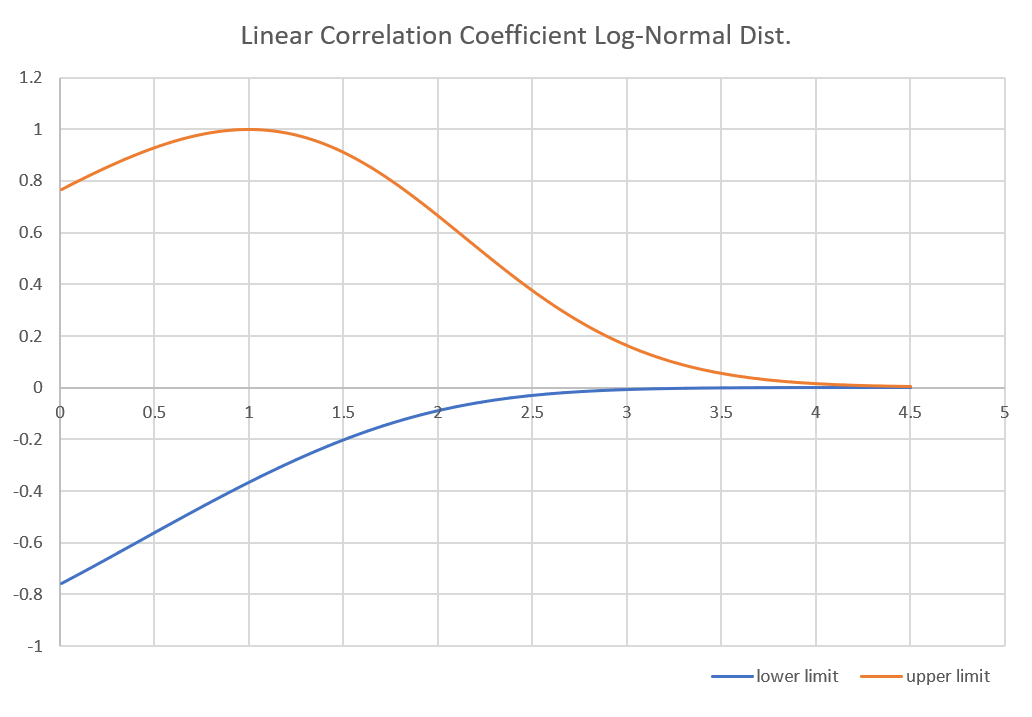
\includegraphics[scale=0.5]{fig/linear_correlation_lognormal.png} 
\end{center}
\end{frame}
%___________________________________________________________________________________________________
%
\subsection{Concordance}

\begin{frame}{Concordance}
   %\footnotesize{
   \begin{itemize}
      \item   				  						  
		Concordance concepts, loosely speaking, aim at capturing the fact that the 
		probability of having "large" (or "small") values of both $X$ and $Y$ is high, while 
		the probability of having "large" values of $X$ together with "small" values of "Y" 
		- or viceversa - is low.
	  \item 
	  	Let $(x, y)^T$ and $(\tilde x, \tilde y)^T$ be two observations from a vector $(X, Y 
	  	)^T$ of continuous random variables. 
	  \item		  	
	  	Then $(x, y)^T$ and $(\tilde x, \tilde y)^T$ 
	  	are said to be concordant if $(x - \tilde x)(y - \tilde y) > 0$, and discordant if $
	  	(x-\tilde x)(y-\tilde y) < 0$.
	  \item 
		The following theorem can be found in Nelsen (1999) p. 127. Many of the results in 	
		this section are direct consequences of this theorem.
   \end{itemize}
 %  }
\end{frame}
%___________________________________________________________________________________________________
%
\begin{frame}{Concordance}
  %\footnotesize{
	\begin{thm}
	Let $(X, Y )^T$ and $(\tilde X, \tilde Y )^T$ be independent vectors of continuous random variables with joint distribution functions $H$ 
	and $\tilde H$, respectively, with common margins $F$ (of $X$ and $\tilde X$) and $G$ (of $Y$ and $\tilde Y$). Let $C$ and $\tilde C
	$ denote the copulas of $(X, Y )^T$ and $(\tilde X, \tilde Y )^T$ respectively,so that $H(x,y)=C(F(x),G(y))$ and $\tilde H(x,y)= \tilde 
	C(F(x),G(y))$. Let $Q$ denote the difference between the probability of concordance and discordance of $(X, Y )^T$ and $(\tilde X, 
	\tilde Y )^T$,  i.e. let
	\begin{equation}
    	Q=\mathbb{P}[(X-\tilde X)(Y-\tilde Y) > 0]-\mathbb{P}[(X-\tilde X)(Y-\tilde Y) < 0] 
	\end{equation}	
	Then
	\begin{equation}
			Q=Q(C, \tilde C) = 4 \iint\limits_{[0,1]^2} \tilde C (u,v) dC(u,v) -1
	\end{equation}
    \end{thm}
 %}
\end{frame}
%___________________________________________________________________________________________________
%
\begin{frame}{Concordance}
\textbf{Proof}. Since the random variables are all continuous,
\footnotesize
$$
\mathbb{P}[(X-\tilde X)(Y-\tilde Y) < 0] = 1 -\mathbb{P}[(X-\tilde X)(Y-\tilde Y) > 0] \Rightarrow Q = 2 
\mathbb{P}[(X-\tilde X)(Y-\tilde Y) > 0] - 1
$$
\normalsize
But
$$
\mathbb{P}[(X-\tilde X)(Y-\tilde Y) > 0] = \mathbb{P}[X > \tilde X, Y > \tilde Y] + \mathbb{P}[X <\tilde X, Y < \tilde Y]
$$
and these probabilities can be evaluated by integrating over the distribution of one of the vectors $(X, Y)^T$ or $(\tilde X, \tilde Y)^T$. Hence

\begin{equation}
\begin{split}
\mathbb{P}[X > \tilde X, Y > \tilde Y] & = \mathbb{P}[ \tilde X < X, \tilde Y < Y] \\
& = \iint\limits_{\mathbb{R}^2} \mathbb{P}[ \tilde X < x, \tilde Y < y] \> dC[F(x), G(y)] \\
& = \iint\limits_{\mathbb{R}^2} \tilde C [F(x), G(y)]  \> dC[F(x), G(y)]
\end{split}
\end{equation}

\end{frame}
%___________________________________________________________________________________________________
%
\begin{frame}{Concordance}
Employing the probability-integral transform $u=F(x)$ and $v = G(y)$ then yields

\begin{equation}
\mathbb{P}[X > \tilde X, Y > \tilde Y] = \mathbb{P}[ \tilde X < X, \tilde Y < Y] 
= \iint\limits_{[0, 1]^2} \tilde C(u, v)  \> dC(u, v)
\end{equation}
Similarly,
\footnotesize
\begin{equation}
\begin{split}
\mathbb{P}[X < \tilde X, Y < \tilde Y] & = \iint\limits_{\mathbb{R}^2} \mathbb{P}[ \tilde X > x, \tilde Y > y] \> dC[F(x), G(y)] \\
& = \iint\limits_{\mathbb{R}^2} \bigl\{1 - F(x) - G(y) + \tilde C[F(x), G(y)]    \bigr\}  \> dC[F(x), G(y)] \\
& = \iint\limits_{[0, 1]^2} \bigl\{1 - u - v + \tilde C(u, v)   \bigr\}  \> dC(u, v)
\end{split}
\end{equation}
\normalsize
\end{frame}
%___________________________________________________________________________________________________
%
\begin{frame}{Concordance}
\footnotesize{
		But since $C$ is the joint distribution function of a vector $(U, V)^T$ of $U(0, 1)$ random variables, $\mathbb{E}(U) = 
		\mathbb{E}(V) = 1/2$, and hence
		
		\begin{equation}
		\mathbb{P}[X < \tilde X, Y < \tilde Y] = 1 - \frac{1}{2} - \frac{1}{2} + \iint\limits_{[0, 1]^2} \tilde C(u, v) \> dC(u, v) =
		\iint\limits_{[0, 1]^2} \tilde C(u, v) \> dC(u, v)
		\end{equation}
		Thus
		
		\begin{equation}
		\mathbb{P}[(X-\tilde X)(Y-\tilde Y) > 0] = 2 \iint\limits_{[0, 1]^2} \tilde C(u, v) \> dC(u, v)
		\end{equation}
		and the conclusion follows
		
		\begin{equation}
		Q = 2 \mathbb{P}[(X-\tilde X)(Y-\tilde Y) > 0] - 1 = 4 \iint\limits_{[0, 1]^2} \tilde C(u, v) \> dC(u, v) - 1
		\end{equation}
}
\end{frame}
%___________________________________________________________________________________________________
%
\subsection{Kendall's tau and Spearman's rho}
\begin{frame}{Kendall's tau and Spearman's rho}

		\textbf{Definition}. Kendall's tau for the random vector $(X, Y)^T$ is defined as
		\begin{equation}
		\tau (X, Y) =\mathbb{P}[(X-\tilde X)(Y-\tilde Y) > 0]-\mathbb{P}[(X-\tilde X)(Y-\tilde Y) < 0] 
		\end{equation}
		where $(\tilde X, \tilde Y)^T$ is an independent copy of $(X, Y)^T$.
		Hence Kendall's tau for $(X, Y)^T$ is simply the probability of concordance minus the probability of discordance and since the 
		copula of  $(\tilde X, \tilde Y)^T$ is the same of $(X, Y)^T$ is also simply equal to $Q(C, C)$:
		
\end{frame}
%___________________________________________________________________________________________________
%
\begin{frame}{Kendall's tau and Spearman's rho}

		\noindent\textbf{Theorem}. Let $(X, Y)^T$ be a vector of continuous random variables with copula $C$. Then Kendall's tau for 
		$(X, Y)^T$ is given by 
		
		\begin{equation}
		\tau (X,Y) = Q(C, C) = 4 \iint\limits_{[0, 1]^2} C(u, v) \> dC(u, v) - 1
		\end{equation}
		
		\noindent Note that the integral above is the expected value of the random variable $C(U, V)$, where $U, V \sim U(0, 1)$ with 
		joint distribution function $C$, i.e. $\tau = 4 \mathbb{E}(C(U,V)) - 1$.

\end{frame}
%___________________________________________________________________________________________________
%
\begin{frame}{Kendall's tau and Spearman's rho}
\footnotesize{
\begin{itemize}
	\item
		\textbf{Definition}.  Spearman's rho for the random vector  $(X, Y)^T$ is defined as
		\begin{equation}
		\rho_S (X, Y) =3 (\mathbb{P}[(X-\tilde X)(Y-Y^\prime) > 0]-\mathbb{P}[(X-\tilde X)(Y-Y^\prime ) < 0]) 
		\end{equation}
		where $(X, Y)^T$, $(\tilde X, \tilde Y)^T$ and $(X^\prime, Y^\prime)^T$ are \textbf{independent} copies.
	\item
		\noindent\textbf{Theorem}.  Let $(X, Y)^T$ be a vector of continuous random variables with copula $C$. Then Spearman's rho 
		for $(X, Y)^T$ is given by (note that $\tilde X$ and $Y^\prime$ are independent so their copula is the product copula)
		\begin{equation}
		\begin{split}
		\rho_S (X, Y) & = 3Q(C, \Pi) = 12 \iint\limits_{[0, 1]^2} uv \> dC(u, v) - 3 = 12 \iint\limits_{[0, 1]^2} C(u,v) \>du\>dv - 3 \\
		& = \frac{\mathbb{E}(UV) - 1/4}{1/12} = \frac{Cov(U, V)}{\sqrt{Var(U)}\sqrt{Var(V)}} \\
		& = \rho[F(X), G(Y)]
		\end{split}
		\end{equation}
\end{itemize}
}
\end{frame}
%===================================================================================================
\section{Copula Families}

\subsection{Gaussian copulas}
\begin{frame}{Elliptical Copulas}
   %\footnotesize{
   \begin{itemize}
      \item  The class of elliptical distributions provides a rich source of multivariate distributions which share many of the tractable 
      properties of the multivariate normal distribution and enables modelling of multivariate extremes and other forms of nonnormal 
      dependences. 
      \item Elliptical copulas are simply the copulas of elliptical distributions. 
      \item Simulation from elliptical distributions is easy, and as a consequence of Sklar’s Theorem so is simulation from elliptical copulas. 		
      \item Furthermore, we will show that rank correlation and tail dependence coefficients can be easily calculated
   \end{itemize}
 %  }
\end{frame}
%___________________________________________________________________________________________________
%
\begin{frame}{Gaussian Copula}
   %\footnotesize{
   \begin{itemize}
      \item The copula of the \textit{n-variate} normal distribution with linear correlation matrix $\rho$ is
		$$
		C_\rho^{Ga} (u_1, \dots, u_2) = \mathbf{\Phi}^d_\rho (\phi^{-1}(u_1), \dots, 
		\phi^{-1}(u_d)) 
		$$
		where $\mathbf{\Phi}^d_\rho$ denotes the joint distribution function of the n-variate standard normal distribution function with 
		linear correlation matrix $\rho$, and $\phi^{-1}$ denotes the inverse of the distribution function of the univariate standard normal 
		distribution. 
		
		\item Copulas of the above form are called Gaussian copulas.
   \end{itemize}
 %  }
\end{frame}
%___________________________________________________________________________________________________
%
\begin{frame}{Gaussian Copula}
   %\footnotesize{
   \begin{itemize}
      \item We now address the question of random variate generation from the Gaussian copula $C_\rho^{Ga} $.
      \item For our purpose, it is sufficient to consider only strictly positive definite matrices $\Sigma$. Write $\Sigma = AA^T$ for some $n 
      \times n$ matrix $A$, and if $Z_1,...,Z_n \sim N(0,1)$ are independent, then $\mu + AZ \sim 
	  N_n(\mu, \Sigma)$.
	 \item One natural choice of $A$ is the Cholesky decomposition of $\Sigma$. The Cholesky decomposition of $\Sigma$ is the unique 
	 lower-triangular matrix $L$ with $LL^T = \Sigma$. Furthermore Cholesky decomposition routines are implemented in most mathematical 
	 software. 
	 \item This provides an easy algorithm for random variate generation from the Gaussian n-copula $C_\rho^{Ga}$.
   \end{itemize}
 %  }
\end{frame}
%___________________________________________________________________________________________________
%
\begin{frame}{Gaussian Copula: Simulation Algorithm}
   %\footnotesize{
   \begin{itemize}
		\item  Find the Cholesky decomposition $A$ of $\Sigma$.
		\item  Simulate $n$ independent random variates $z_1, . . . , z_n$ from $N (0, 1)$.
		\item  Set $x=Az$.
		\item  Set $u_i = \Phi(x_i), \quad i = 1,...,n$.
		\item  $(u_1,...,u_n)^T\sim C_\rho^{Ga}$
	\end{itemize}
	\vspace{2em}
	As usual $\Phi$ denotes the univariate standard normal distribution function.
 %  }
\end{frame}
%___________________________________________________________________________________________________
%
\begin{frame}{Gaussian Copula with Gaussian Marginals ($\rho = 0.2$)}
    \begin{figure}[ht]
        \begin{minipage}[b]{0.45\linewidth}
            \centering
            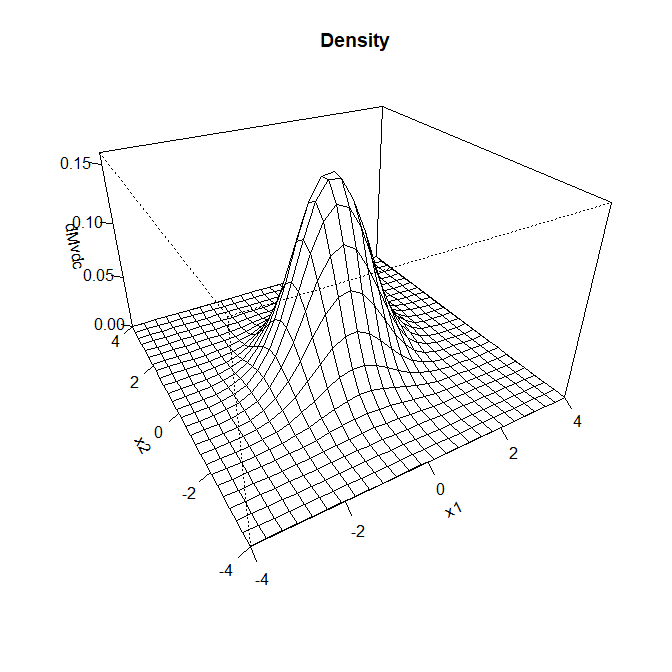
\includegraphics[width=\textwidth]{fig/gauss_gauss_density_0_2.png}
            %\caption{a) Densità}
            %\label{fig:a}
        \end{minipage}
        \hspace{0.5cm}
        \begin{minipage}[b]{0.45\linewidth}
            \centering
            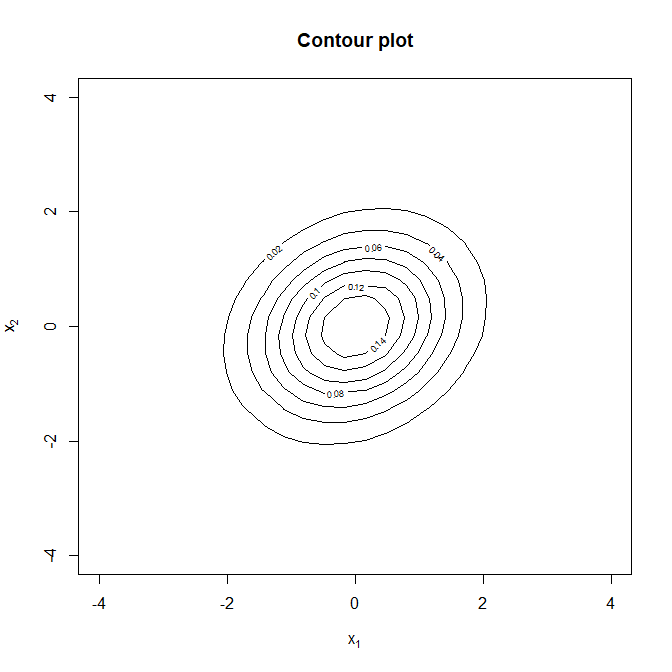
\includegraphics[width=\textwidth]{fig/gauss_gauss_contour_0_2.png}
            %\caption{b) Contour Plot}
            %\label{fig:b}
        \end{minipage}
    \end{figure}
\end{frame}
%___________________________________________________________________________________________________
%
\begin{frame}{Gaussian Copula with $t_\nu$ Marginals ($\rho = 0.2$)}
    \begin{figure}[ht]
        \begin{minipage}[b]{0.45\linewidth}
            \centering
            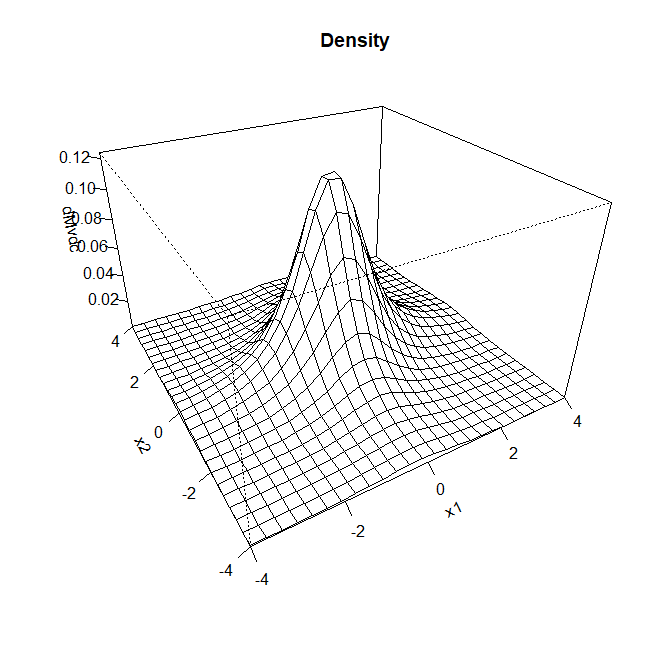
\includegraphics[width=\textwidth]{fig/gauss_t_density_0_2.png}
            %\caption{a) Densità}
            %\label{fig:a}
        \end{minipage}
        \hspace{0.5cm}
        \begin{minipage}[b]{0.45\linewidth}
            \centering
            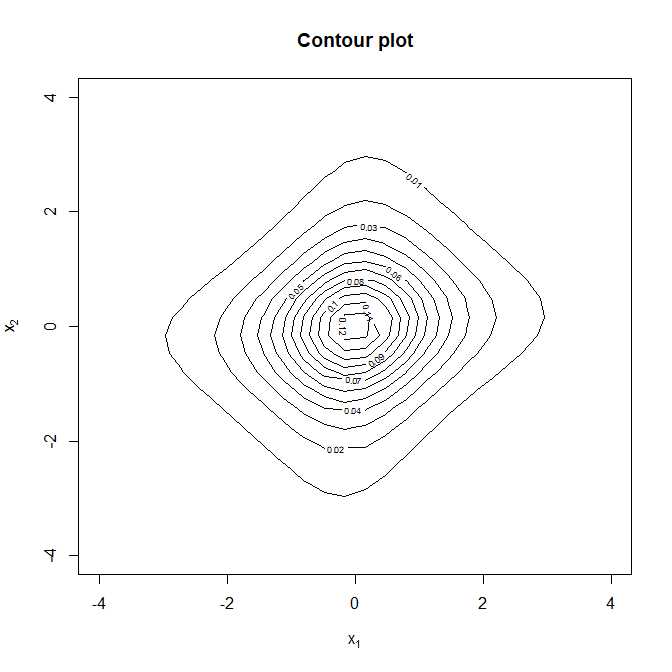
\includegraphics[width=\textwidth]{fig/gauss_t_contour_0_2.png}
            %\caption{b) Contour Plot}
            %\label{fig:b}
        \end{minipage}
    \end{figure}
\end{frame}
%___________________________________________________________________________________________________
%
\begin{frame}{Gaussian Copula with Gaussian Marginals ($\rho = 0.9$)}
    \begin{figure}[ht]
        \begin{minipage}[b]{0.45\linewidth}
            \centering
            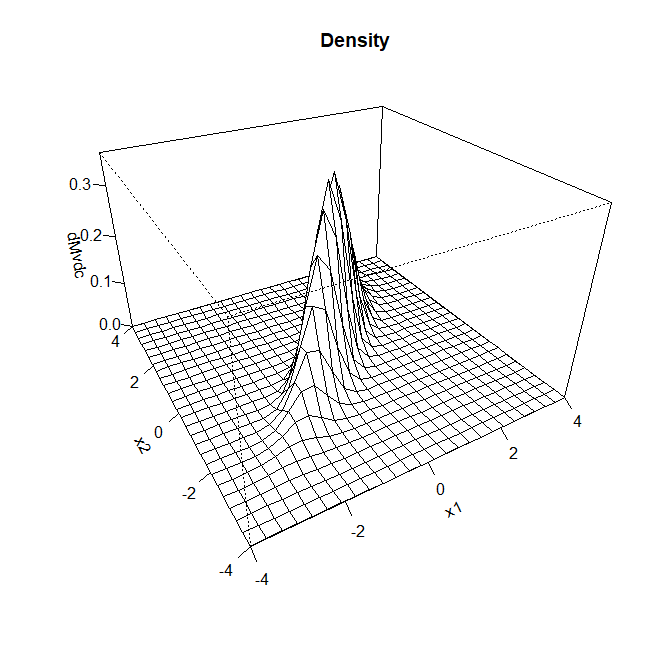
\includegraphics[width=\textwidth]{fig/gauss_gauss_density_0_9.png}
            %\caption{a) Densità}
            %\label{fig:a}
        \end{minipage}
        \hspace{0.5cm}
        \begin{minipage}[b]{0.45\linewidth}
            \centering
            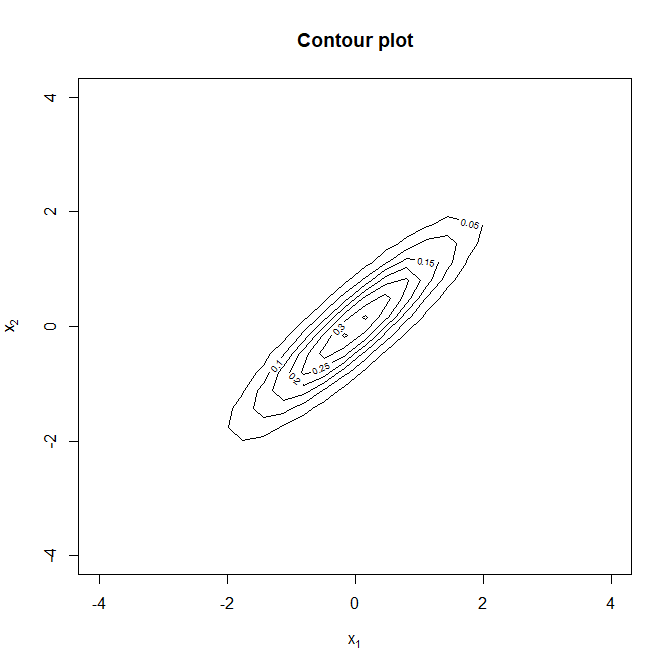
\includegraphics[width=\textwidth]{fig/gauss_gauss_contour_0_9.png}
            %\caption{b) Contour Plot}
            %\label{fig:b}
        \end{minipage}
    \end{figure}
\end{frame}
%___________________________________________________________________________________________________
%
\begin{frame}{Gaussian Copula with $t_\nu$ Marginals ($\rho = 0.9$)}
    \begin{figure}[ht]
        \begin{minipage}[b]{0.45\linewidth}
            \centering
            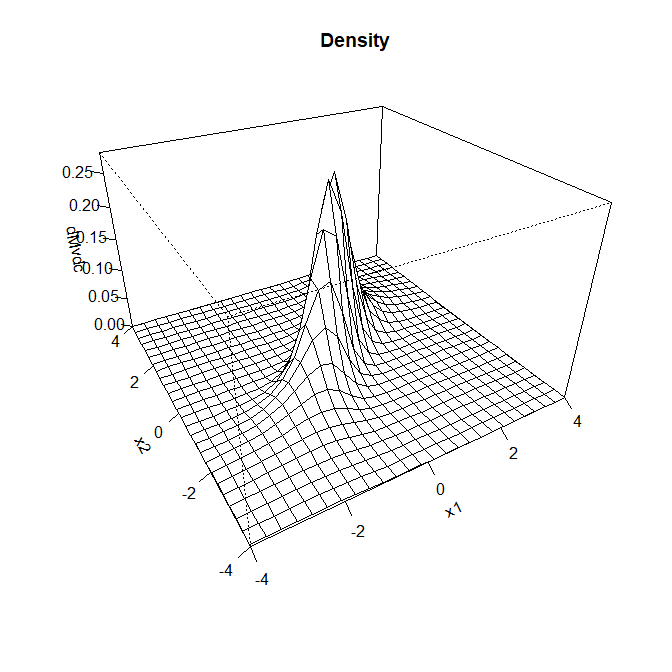
\includegraphics[width=\textwidth]{fig/gauss_t_density_0_9.png}
            %\caption{a) Densità}
            %\label{fig:a}
        \end{minipage}
        \hspace{0.5cm}
        \begin{minipage}[b]{0.45\linewidth}
            \centering
            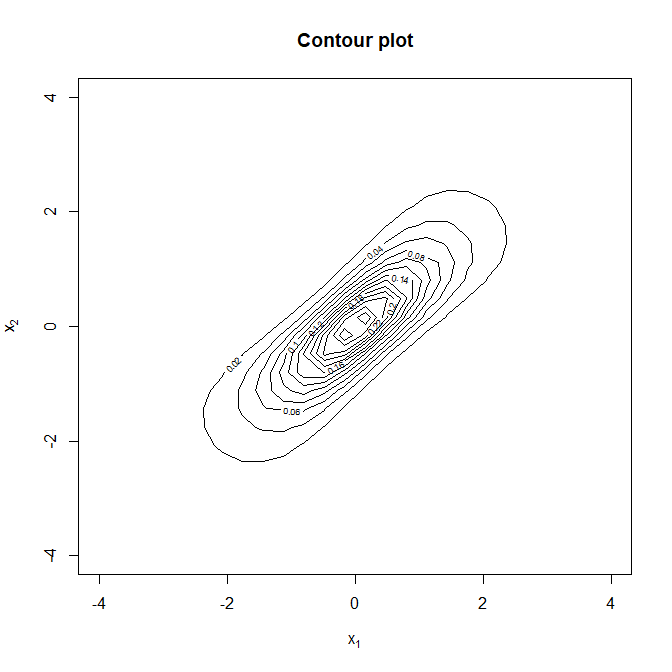
\includegraphics[width=\textwidth]{fig/gauss_t_contour_0_9.png}
            %\caption{b) Contour Plot}
            %\label{fig:b}
        \end{minipage}
    \end{figure}
\end{frame}

\subsection{t-copulas}
%___________________________________________________________________________________________________
%
\begin{frame}{t copula}
\footnotesize{
   \begin{itemize}
    \item 
    	Similarly to the case of a normal distribution we can consider the distribution 
    	$t_\nu$; the corresponding copula with correlation $\rho$ is:
		\begin{equation}
						C^t_{\nu, \rho}(u_1,\dots,u_d) = \Theta^d_{\nu, \rho} 
						(t^{-1}_\nu(u_1),\dots,t^{-1}_\nu(u_d))
		\end{equation}
		where $\Theta^d_{\nu, \rho}$ is the $t$ multivariate distribution with dimension $d
		$, $\nu$ degree of freedom and linear correlation $\rho$ while $t^{-1}_\nu$ is the 
		inverse univariate standard t-distribution $t_\nu$.
	\item 
		Also for this functional you have a simple simulation algorithm based on the 
		following result: If X has the stochastic representation
		$$
			X=\frac{\sqrt{\nu}}{\sqrt{Z}}Y \quad \text{with} \quad Y \sim \mathcal{N}_d(0,
			\rho), Z \sim \chi^2_\nu 
		$$
		then $X$ has an $n-variate$ $t_\nu$-distribution with mean $\mu$ (for $\nu > 1$) and 
		covariance matrix $\nu \Sigma/(\nu-2)$ (for $\nu > 2$). If $\nu \le 2$ then $Cov(X)$ 
		is not defined. In this case we just interpret $\Sigma$ as being the shape parameter 
		of the distribution of $X$.
   \end{itemize}
}
\end{frame}
%___________________________________________________________________________________________________
%
\begin{frame}{t copula: Simulation Algorithm}
   %\footnotesize{
   \begin{itemize}
		\item Find the Cholesky decomposition $A$ of $\Sigma$.
		\item Simulate $n$ independent random variates $z_1, . . . , z_n$ from $N (0, 1)$.
		\item Simulate a random variate $s$  from $\chi^2_\nu$ independent of $z_1, . . . , 
		z_n$.
		\item Set $x=Az$
		\item Set $y = \sqrt{\frac{n}{s}} x$ 
		\item Set $u_i = T_\nu(y_i)$ for $i=1,\dots,n$
		\item $(u_1,...,u_n)^T \sim C^t_{\nu, \Sigma}$.   
   \end{itemize}
 %  }
\end{frame}

\subsection{Archimedean copulas}
%___________________________________________________________________________________________________
%
\begin{frame}{Archimedean copulas}
   %\footnotesize{
   \begin{itemize}
      \item In this section we discuss an important class of copulas called Archimedean copulas. 
      \item They have proved to be useful in several applications since they are capable of capturing wide ranges of dependence 
      structures. 
      \item Furthermore, in contrast to elliptical copulas, all commonly encountered Archimedean copulas have closed form expressions.
      \item We divide the discussion of Archimedean copulas in two subsections: the first introduces them and their main properties 
      while the second presents different one-parameter families of Archimedean copulas.
\end{itemize}
 %  }
\end{frame}
%___________________________________________________________________________________________________
%
\begin{frame}{Archimedean copulas}
\begin{itemize}
\item
Archimedean copulas may be constructed using a function $\phi : \mathbb{I} \rightarrow [0, \infty]$, 
continuous, decreasing, convex and such that $\phi(1) = 0$. 
\item
Such a function $\phi$ is called a generator. It is called a strict generator whenever $\phi(0) = +\infty$. 
\item
The pseudo-inverse of $\phi$ is defined as follows:
\end{itemize}
\begin{center}
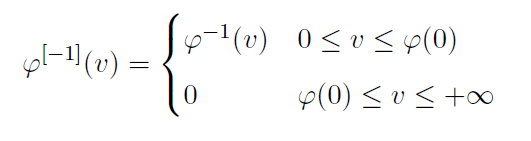
\includegraphics[scale=.5]{fig/copule_archimedee_pseudoinv.PNG} 
\end{center}
\end{frame}
%___________________________________________________________________________________________________
%
\begin{frame}{Archimedean copulas}


The pseudo-inverse is such that, by composition with the generator, it gives the identity, and it coincides with the usual      
	inverse if $\phi$ is a strict generator. \\[2ex]

\noindent\textbf{Definition} Given a generator and its pseudo-inverse, an Archimedean 2-copula takes the form
\begin{equation}
C(u, v) = \phi^{[-1]}\Bigl( \phi(u) + \phi(v) \Bigr)
\end{equation}

If the generator is strict, the copula is said to be a strict Archimedean 2-copula.				  						  

\end{frame}
%___________________________________________________________________________________________________
%
\begin{frame}{Archimedean copulas}
\begin{center}
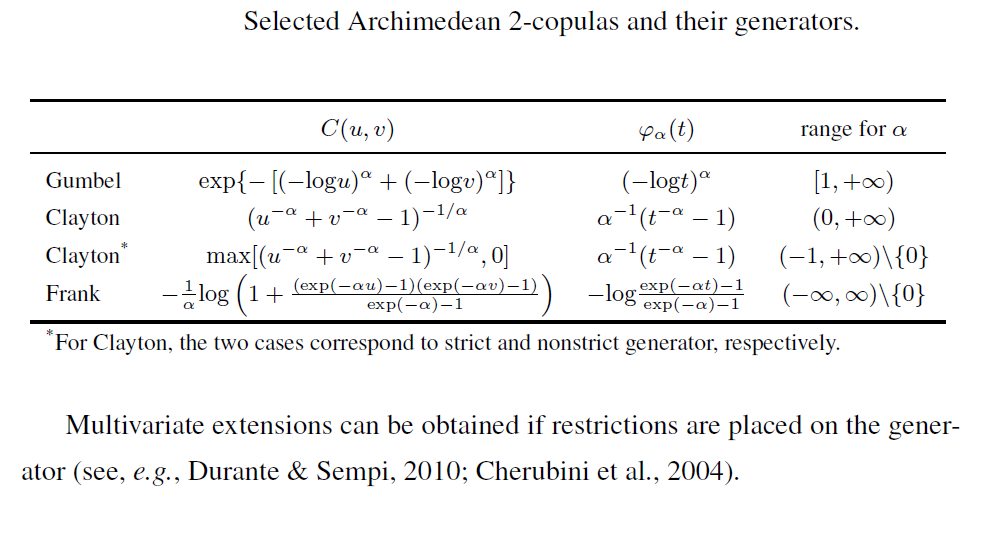
\includegraphics[scale=.45]{fig/copule_archimedee_tabella.PNG} 
\end{center}
\end{frame}
%___________________________________________________________________________________________________
%
\begin{frame}{Archimedean copulas: Gumbel \textit{d}-copula}
		The Gumbel family has been introduced by Gumbel (1960). Since it has been discussed in Hougaard (1986), it is also known as 
		the Gumbel–Hougaard family. The standard expression for members of this family of d-copulas is
		\begin{center}
		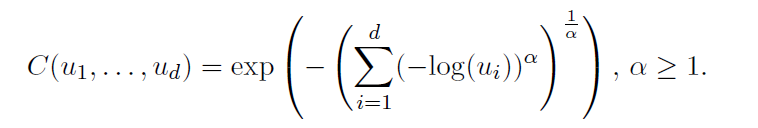
\includegraphics[scale=.5]{fig/copule_archimedee_gumbel.PNG} 
		\end{center}
		The case $\alpha = 1$ gives the product copula as a special case, and the limit for $\alpha \rightarrow +\infty$ is the 
		comonotonicity copula. It follows that the Gumbel family can represent independence and positive dependence only. The 
		generator is given by 
		\begin{equation}
		\phi_\alpha(u) = \bigl( -\log \> u \bigr)^\alpha, \quad \alpha \ge 1
		\end{equation}
\end{frame}
%___________________________________________________________________________________________________
%
\begin{frame}{Archimedean copulas: Clayton \textit{d}-copula}
		 The Clayton family was first proposed by Clayton (1978), and studied by Oakes (1982). The standard expression for members 
		 of this family of d-copulas is
		 \begin{center}
		 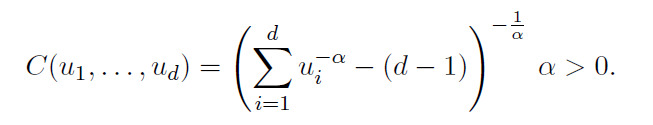
\includegraphics[scale=.5]{fig/copule_archimedee_clayton.PNG} 
		 \end{center}
		 The limiting case $\alpha = 0$ corresponds to the independence copula. The generator has the form 
		 \begin{equation}
		 \phi_\alpha(u) = u^{-\alpha}-1, \quad \alpha > 0
		\end{equation}
 \end{frame}
%___________________________________________________________________________________________________
%
\begin{frame}{Archimedean copulas: Frank \textit{d}-copula}
		Copulas of this family have been introduced by Frank (1979), and have the expression:
		\begin{center}
		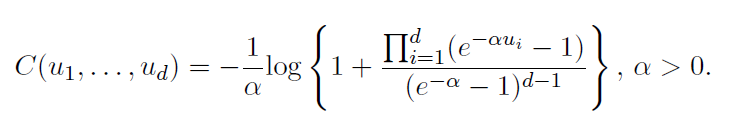
\includegraphics[scale=.5]{fig/copule_archimedee_frank_1.PNG} 
		\end{center}
		It reduces to the product copula if $\alpha = 0$. For the case $d = 2$, the parameter $\alpha$ can be extended also to 
		the case $\alpha < 0$. The generator is given by
		\begin{center}
		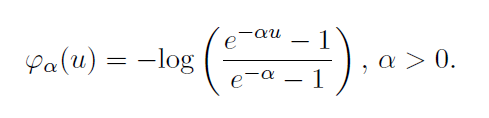
\includegraphics[scale=.5]{fig/copule_archimedee_frank_2.PNG} 
		\end{center}
\end{frame}
%___________________________________________________________________________________________________
%
\begin{frame}{Bivariate sample from the Gumbel copula}
	\begin{center}
	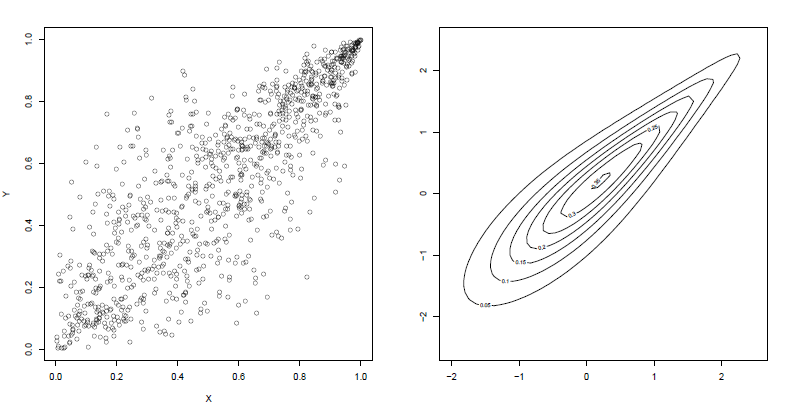
\includegraphics[scale=.5]{fig/copule_archimedee_gumbel_plot.PNG} 	
	\end{center}
\end{frame}
%___________________________________________________________________________________________________
%
\begin{frame}{Bivariate sample from the Clayton copula}
	\begin{center}
	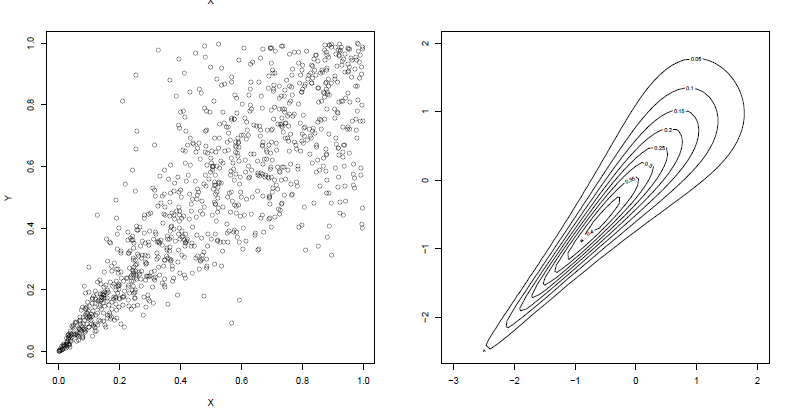
\includegraphics[scale=.5]{fig/copule_archimedee_clayton_plot.PNG} 	
	\end{center}
\end{frame}
%___________________________________________________________________________________________________
%
\begin{frame}{Bivariate sample from the Frank copula}
	\begin{center}
	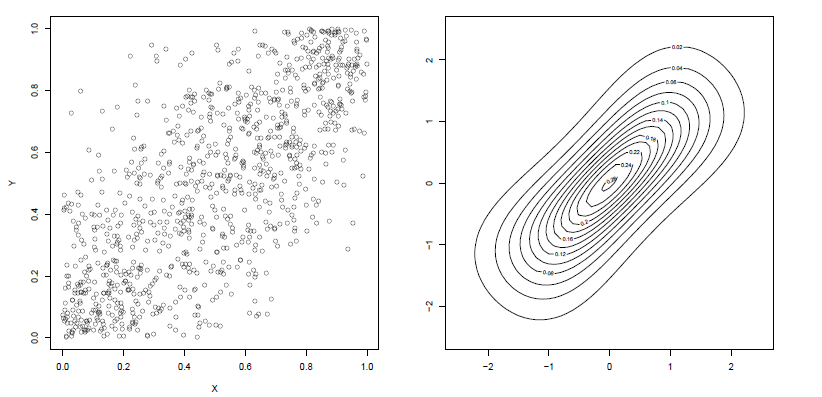
\includegraphics[scale=.5]{fig/copule_archimedee_frank_plot.PNG} 	
	\end{center}
\end{frame}
%===================================================================================================
\section{Tail Dependence}
%___________________________________________________________________________________________________
%
\begin{frame}{Titolo}
%\footnotesize{
   \begin{itemize}
		\item item 1 
		\item item 2
		\item item 3
	\end{itemize}
 % }
\end{frame}

\end{document}
